%%%%%%%%%%%%%%%%%%%%%%%%%%%%%%%%%%%%%%%%%
% Beamer Presentation
% LaTeX Template
% Version 1.0 (10/11/12)
%
% This template has been downloaded from:
% http://www.LaTeXTemplates.com
%
% License:
% CC BY-NC-SA 3.0 (http://creativecommons.org/licenses/by-nc-sa/3.0/)
%
%%%%%%%%%%%%%%%%%%%%%%%%%%%%%%%%%%%%%%%%%

%----------------------------------------------------------------------------------------
%	PACKAGES AND THEMES
%----------------------------------------------------------------------------------------

\documentclass{beamer}

\mode<presentation> {

% The Beamer class comes with a number of default slide themes
% which change the colors and layouts of slides. Below this is a list
% of all the themes, uncomment each in turn to see what they look like.

%\usetheme{default}
%\usetheme{AnnArbor}
%\usetheme{Antibes}
%\usetheme{Bergen}
%\usetheme{Berkeley}
%\usetheme{Berlin}
%\usetheme{Boadilla}
%\usetheme{CambridgeUS}
%\usetheme{Copenhagen}
\usetheme{Darmstadt}
%\usetheme{Dresden}
%\usetheme{Frankfurt}
%\usetheme{Goettingen}
%\usetheme{Hannover}
%\usetheme{Ilmenau}
%\usetheme{JuanLesPins}
%\usetheme{Luebeck}
%\usetheme{Madrid}
%\usetheme{Malmoe}
%\usetheme{Marburg}
%\usetheme{Montpellier}
%\usetheme{PaloAlto}
%\usetheme{Pittsburgh}
%\usetheme{Rochester}
%\usetheme{Singapore}
%\usetheme{Szeged}
%\usetheme{Warsaw}

% As well as themes, the Beamer class has a number of color themes
% for any slide theme. Uncomment each of these in turn to see how it
% changes the colors of your current slide theme.

%\usecolortheme{albatross}
\usecolortheme{beaver} %great
%\usecolortheme{beetle}
%\usecolortheme{crane}
%\usecolortheme{dolphin}
%\usecolortheme{dove} %great
%\usecolortheme{fly}
%\usecolortheme{lily}
%\usecolortheme{orchid}
%\usecolortheme{rose}
%\usecolortheme{seagull}
%\usecolortheme{seahorse}
%\usecolortheme{whale}
%\usecolortheme{wolverine}

%\setbeamertemplate{footline} % To remove the footer line in all slides uncomment this line
%\setbeamertemplate{footline}[page number] % To replace the footer line in all slides with a simple slide count uncomment this line

%\setbeamertemplate{navigation symbols}{} % To remove the navigation symbols from the bottom of all slides uncomment this line
}

\usepackage{graphicx} % Allows including images
\usepackage{booktabs} % Allows the use of \toprule, \midrule and \bottomrule in tables
\usepackage{bbm}
\usepackage{amssymb,amsmath}
\usepackage{soul}
\usepackage{sansmathaccent}
\pdfmapfile{+sansmathaccent.map}

%----------------------------------------------------------------------------------------
%	TITLE PAGE
%----------------------------------------------------------------------------------------

\title[Manage the Data from Indoor Spaces]{Manage the Data from Indoor Spaces: \\Models, Indexes \& Query Processing} % The short title appears at the bottom of every slide, the full title is only on the title page

\author{Huan Li} % Your name
\institute[Zhejiang University] % Your institution as it will appear on the bottom of every slide, may be shorthand to save space
{
Database Laboratory, Zhejiang University \\ % Your institution for the title page
\medskip
\textit{lihuancs@zju.edu.cn} % Your email address
}
\date{\today} % Date, can be changed to a custom date

\begin{document}

\begin{frame}
\titlepage % Print the title page as the first slide
\end{frame}

\begin{frame}
\frametitle{Overview} % Table of contents slide, comment this block out to remove it
\setcounter{tocdepth}{1}
\tableofcontents % Throughout your presentation, if you choose to use \section{} and \subsection{} commands, these will automatically be printed on this slide as an overview of your presentation
\end{frame}

\AtBeginSection[]
{
    \begin{frame}[shrink]
        \tableofcontents[sectionstyle=show/shaded,subsectionstyle=show/shaded/hide]
    \end{frame}
}

%----------------------------------------------------------------------------------------
%	PRESENTATION SLIDES
%----------------------------------------------------------------------------------------

%------------------------------------------------
\section{1. Outlines} % Sections can be created in order to organize your presentation into discrete blocks, all sections and subsections are automatically printed in the table of contents as an overview of the talk
%------------------------------------------------

%------------------------------------------------

\begin{frame}
\frametitle{Aims}
\begin{itemize}
\item To give a brief review introduction to \emph{indoor data management techniques}.
\\~\\
\item To review a series of works in this field, including their proposed \emph{models}, \emph{indexes} and \emph{algorithms}.
\\~\\
\item To discuss how to bring those advanced theoretical contents into practice.
\end{itemize}
\end{frame}

%------------------------------------------------
\section{2. Indoor Space Models \& Applications} % Sections can be created in order to organize your presentation into discrete blocks, all sections and subsections are automatically printed in the table of contents as an overview of the talk
%------------------------------------------------

\subsection{2.1 Graph Model Based Indoor Tracking} % A subsection can be created just before a set of slides with a common theme to further break down your presentation into chunks

\begin{frame}
\frametitle{About This Work...}
\emph{Graph Model Based Indoor Tracking}.~\cite{DBLP:conf/mdm/JensenLY09} \\ C.~S. Jensen, H.~Lu, and B.~Yang.\\~\\
\begin{itemize}
\item Published in year 2009, \emph{MDM} conference.
\item A pioneering work that introduces base graph model to indoor data management.
\item Detailed tracking algorithms are designed for RFID-based positioning.
\item Easy to understand, with comprehensive concepts.
\end{itemize}

\end{frame}

%------------------------------------------------

\begin{frame}
\frametitle{Motivation}
\begin{itemize}
\item We are spending most of our time in indoor spaces
    \begin{itemize}
    \item Office building, University, Shopping Centers, etc.
    \end{itemize}
\item We cannot use GPS-based tracking indoor movements
    \begin{itemize}
    \item Indoor navigation and route guidance (museum)
    \item Flow analysis
        \begin{itemize}
        \item how do people use the indoor space $\rightarrow$ important in pricing of advertisement space in store rental
        \end{itemize}
    \end{itemize}
\item We can use other technology...
    \begin{itemize}
    \item Wi-Fi, Infrared, Bluetooth or RFID
    \item This paper is focusing on RFID, since it is now mature and effortless
    \item RFID tags are cheap and RFID reader are expensive
    \end{itemize}
\end{itemize}

\end{frame}

\begin{frame}
\frametitle{Idea}

\begin{columns}[c]

\column{.6\textwidth}
\begin{figure}[tb]
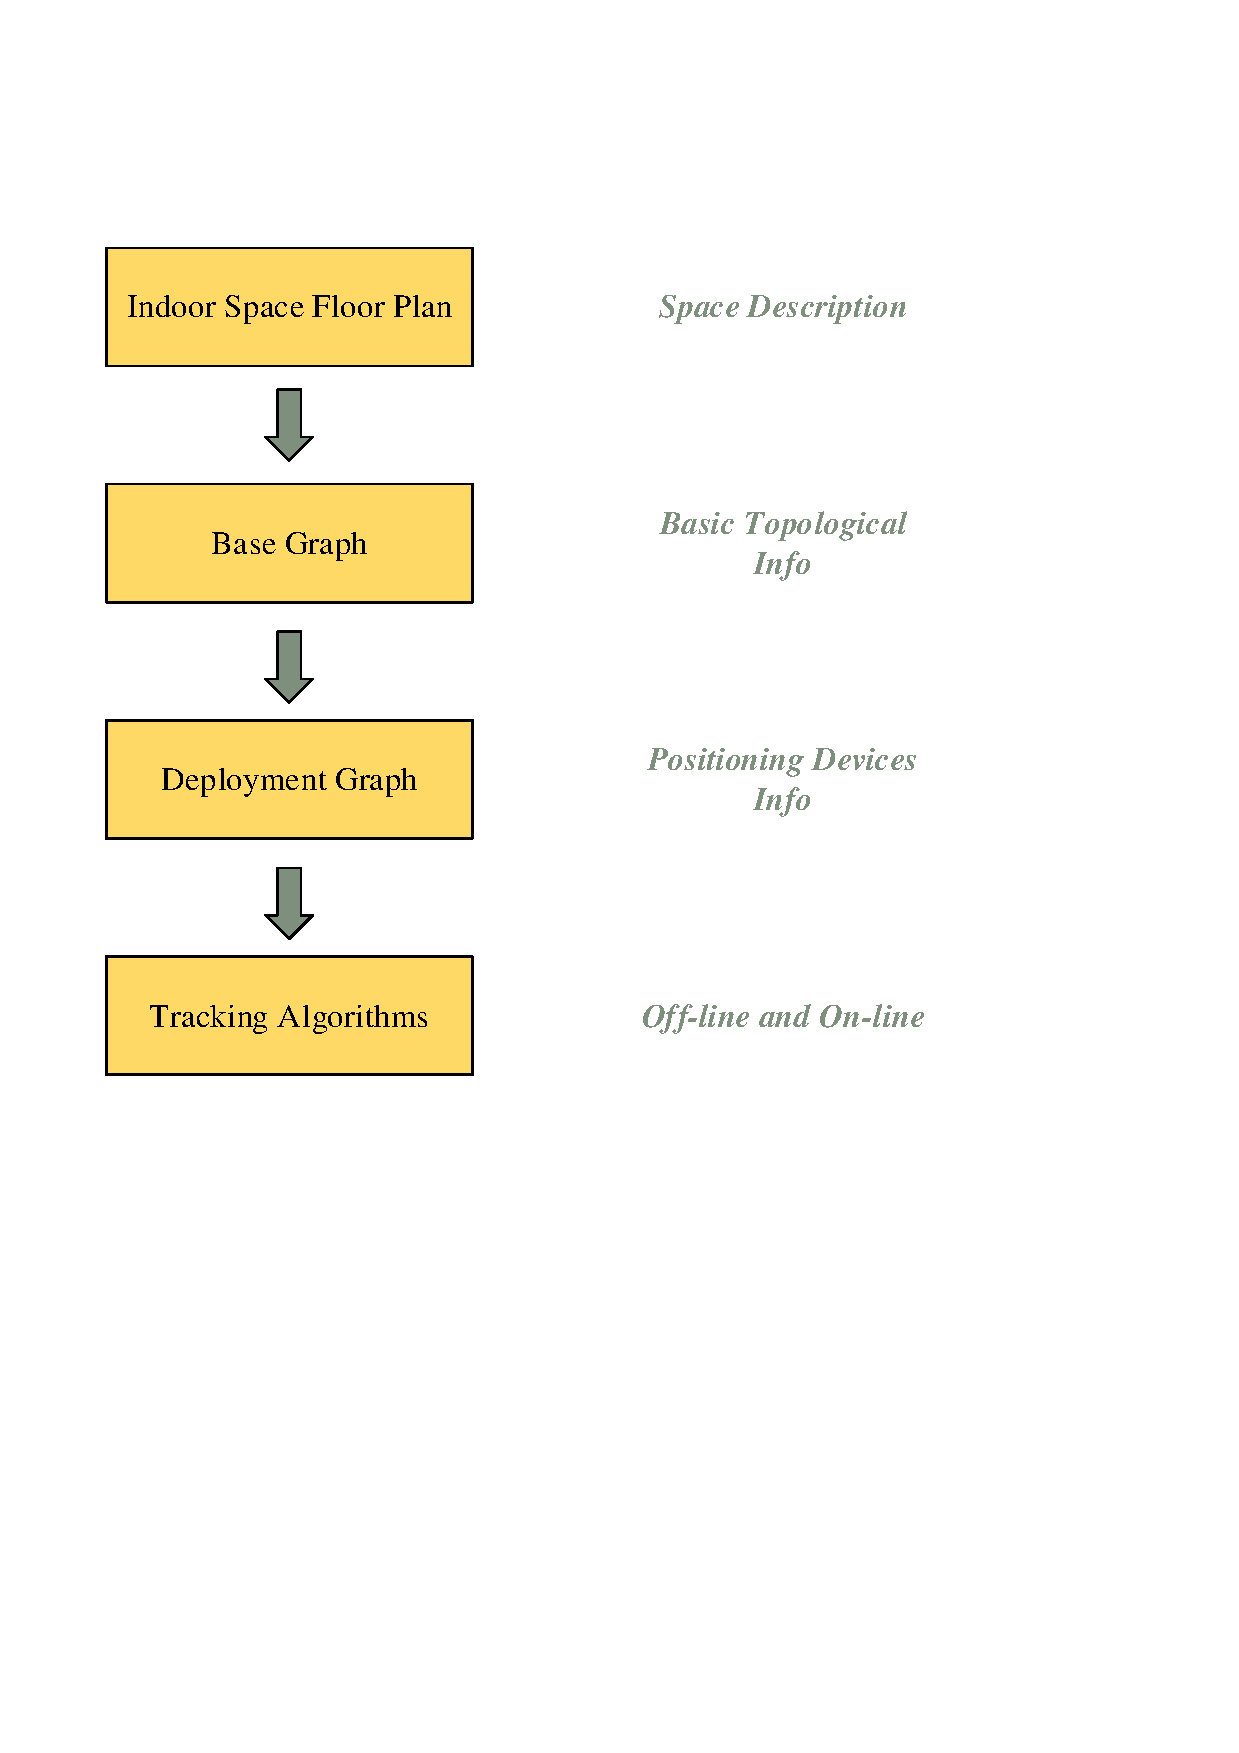
\includegraphics[width=\columnwidth]{figures/2-1-1.pdf}
\end{figure}

\column{.4\textwidth}
\pause \textbf{Goal:} \textrm{Improve indoor tracking accuracy from a data management perspective, to capture where a particular object can be at a particular time.}

\end{columns}
\end{frame}

\begin{frame}
\frametitle{Base Graph Model}

\small{By capturing the essential connectivity and accessibility, \textbf{Base Graph} describes the topology of a floor plan of a possibly complex indoor space.}

\begin{columns}[c]

\column{.45\textwidth}
\begin{figure}[tb]
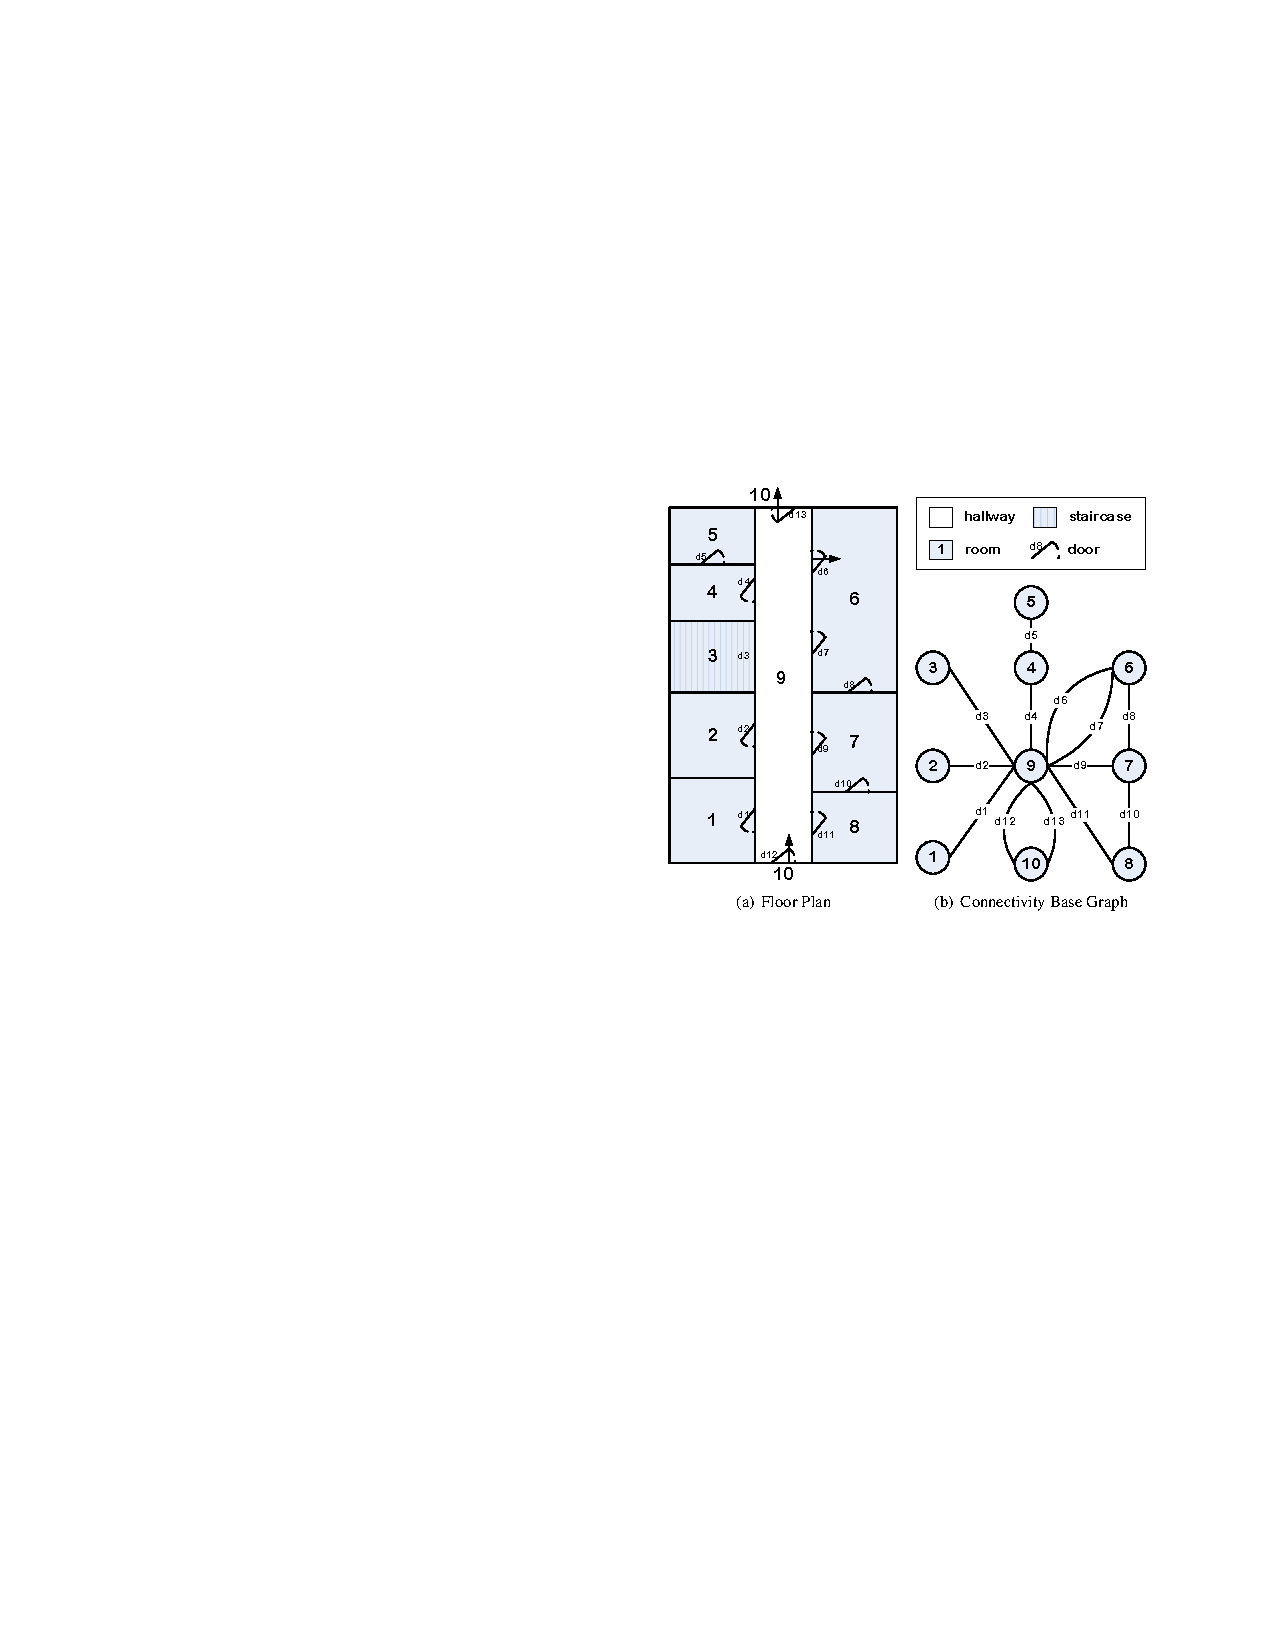
\includegraphics[width=\columnwidth]{figures/2-1-2.pdf}
\end{figure}

\column{.55\textwidth}
\begin{block}{Connectivity Base Graph}
a labeled, undirected graph.
\textrm{
\begin{itemize}
\item $\mathnormal{G_{conn} = \{V, E_d, \Sigma_{door}\}}$
\item $\mathnormal{V}$: each separate partition is represented as a vertex
\item $\mathnormal{E_d}$: each door is captured as an edge%, i.e., $\mathnormal{(\{v_i,v_j}, k)}$
\item $\mathnormal{\Sigma_{door}}$: a set of edge labels that represent connections
\end{itemize}
}
\end{block}

\end{columns}
\end{frame}

%------------------------------------------------


\begin{frame}
\frametitle{Base Graph Model}

\small{\textbf{Accessibility Graph} is constructed to represent the movement permitted by doors or connections.}

\begin{columns}[c]

\column{.45\textwidth}
\begin{figure}[tb]
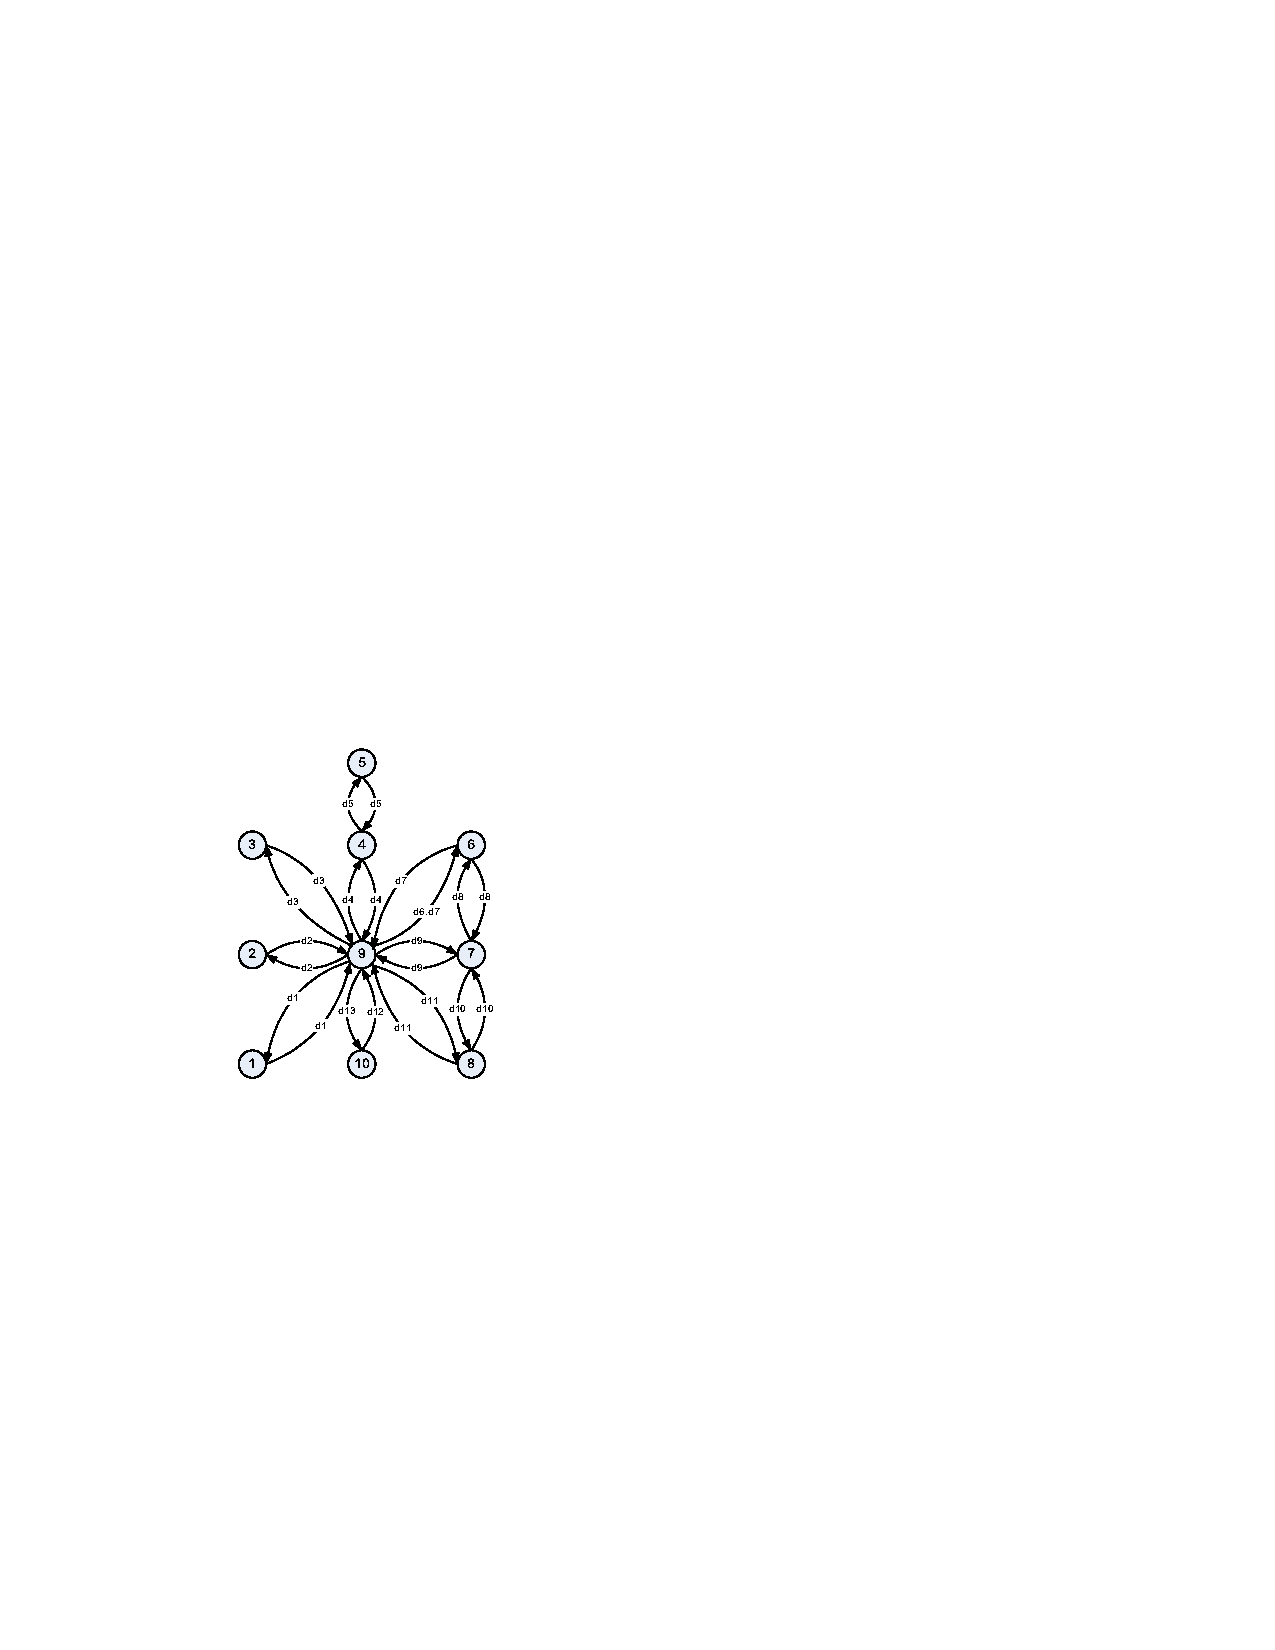
\includegraphics[width=\columnwidth]{figures/2-1-3.pdf}
\end{figure}

\column{.55\textwidth}
\begin{block}{Accessibility Graph}
a labeled, directed graph.
\textrm{
\begin{itemize}
\item $\mathnormal{G_{accs} = \{V, E, \Sigma_{door}, l_e\}}$
\item $\mathnormal{V}$: the set of vertices
\item $\mathnormal{E}$: the set of directed edges, i.e., $\mathnormal{E=\{\langle v_i, v_j\rangle | v_i, v_j \in V \wedge v_i \neq v_j\}}$
\item $\mathnormal{l_e}$: a function that maps edges to subsets of the set of doors, i.e., $\mathnormal{l_e : E \rightarrow 2^{\Sigma_{door}}}$
\end{itemize}
}
\end{block}

\end{columns}
\end{frame}

%------------------------------------------------


\begin{frame}
\frametitle{Base Graph Model}

\small{In addition to the topological information of a floor plan, its geometrical information should also be captured.}
\\~\\
\pause

The \textrm{\em Building Partitions Mapping} is defined as:
\pause
\begin{equation}
\mathnormal{BuildingPartitions: V \rightarrow Ploygons}
\end{equation}
\\~\\
\pause

The \textrm{\em Doors Mapping} is defined as:
\pause
\begin{equation}
\mathnormal{Doors: \Sigma_{door} \rightarrow Line~Segments}
\end{equation}

\end{frame}

%------------------------------------------------


\begin{frame}
\frametitle{RFID Deployment Graph Model}
\begin{itemize}
\item RFID based proximity analysis
    \begin{itemize}
    %\item a record is produced when a \emph{RFID tag} approaches a \emph{RFID reader}.
    \item RFID readers deployment may cover only part of the space, or it may be capable of only detecting some movements in the space.
    \item assume that all RFID readers have disjoint activation ranges.
    \end{itemize}
\item Types of RFID readers
    \begin{itemize}
    \item \textbf{Partitioning Readers} partition the indoor space into cells in the sense that an object cannot move from one cell to another without being observed.
    \item \textbf{Presence Readers} simply observe the presence(and non-presence) of tags in their activation ranges.
    \end{itemize}
\end{itemize}
\end{frame}

%------------------------------------------------


\begin{frame}
\frametitle{RFID Deployment Graph Model}

\small{Vertices represent cells. A directed edge indicates that one can move from one cell to another without entering other cells, which is detected by a corresponding partitioning reader.}
\begin{columns}[c]

\column{.45\textwidth}
\begin{figure}[tb]
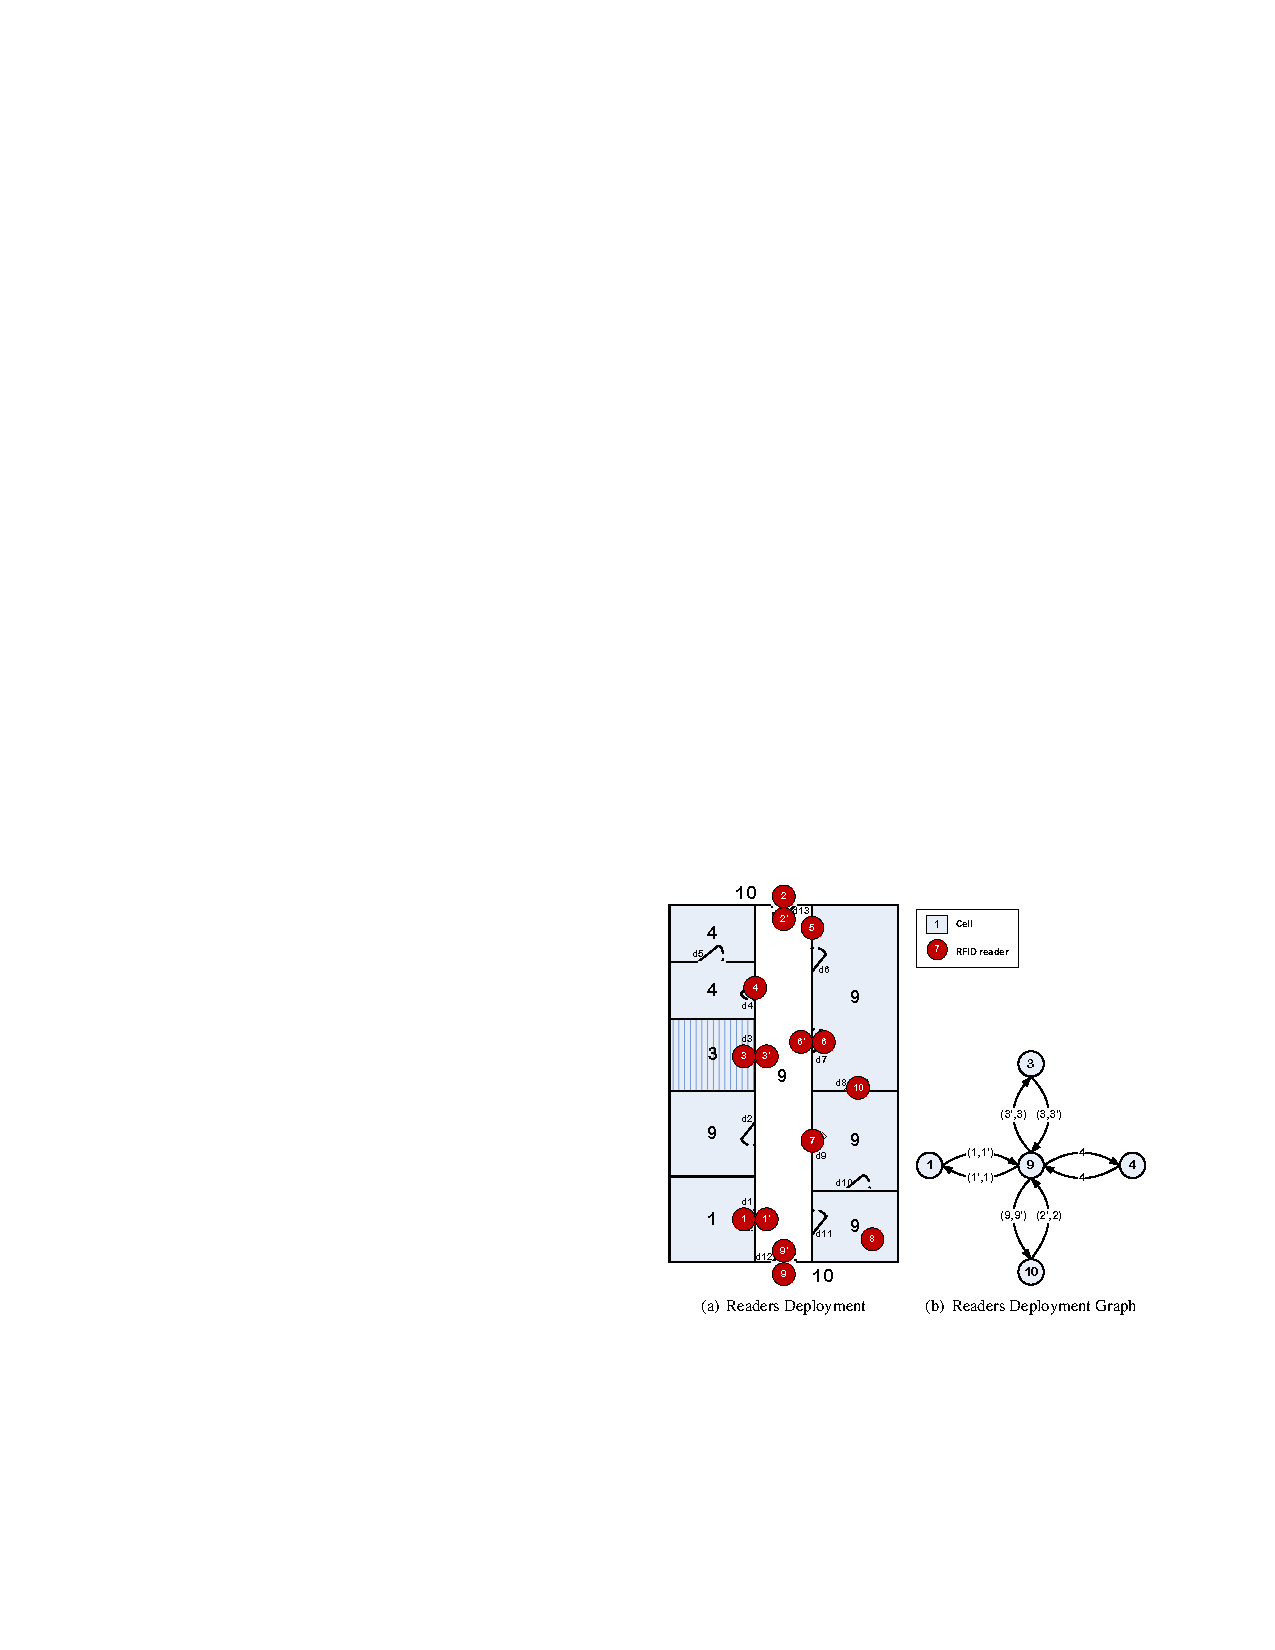
\includegraphics[width=\columnwidth]{figures/2-1-4.pdf}
\end{figure}

\column{.55\textwidth}
\begin{block}{RFID Deployment Graph}
a labeled, directed graph.
\textrm{
\begin{itemize}
\item $\mathnormal{G_{RFID} = \{C, E_r, \Sigma_{reader}, l_e\}}$
\item $\mathnormal{C}$: the set of the vertices
\item $\mathnormal{E_r}$: An edge is an ordered pair $\mathnormal{\langle c_i, c_j \rangle}$ of distinct vertices from $\mathnormal{C}$
\item $\mathnormal{l_e}$ maps an edge to a partitioning reader (pair), i.e., $\mathnormal{E_r \rightarrow 2^{\Sigma_{reader}} \cup 2^{\Sigma_{reader} \times \Sigma_{reader}}}$
\end{itemize}
}
\end{block}

\end{columns}
\end{frame}

\begin{frame}
\frametitle{RFID Deployment Graph Construction}

\small{Each cell created by partitioning readers corresponds to one or more base graph partitions.}
\pause
\begin{equation}
\mathnormal{Cells: V \rightarrow C}
\end{equation}
\\~\\
\pause

\small{For each RFID reader, record its accurate deployment location and activation range.}
\pause
\begin{equation}
\mathnormal{
\begin{aligned}
Mapping~1: &\Sigma_{reader} \rightarrow \{ (loc, range, flag) | loc \in R^2 \wedge \\
  &range \in (0,d_{max}] \wedge flag \in {PAR, PRE} \}
\end{aligned}
}
\end{equation}
\\~\\
\pause

\small{A mapping of readers to the cells that their activation ranges intersect is introduced:}
\pause
\begin{equation}
\mathnormal{
Mapping~2: \Sigma_{reader} \rightarrow 2^C
}
\end{equation}

\end{frame}

%------------------------------------------------

%------------------------------------------------

\subsection{2.2 Scalable Continuous Range Monitoring of Moving Objects in Symbolic Indoor Space} % A subsection can be created just before a set of slides with a common theme to further break down your presentation into chunks

\begin{frame}
\frametitle{Motivation}
Scalable Continuous Range Monitoring of Moving Objects in Symbolic Indoor Space.~\cite{DBLP:conf/cikm/YangLJ09}\\~\\


\end{frame}

%------------------------------------------------

\subsection{2.3 Probabilistic Threshold k Nearest Neighbor Queries over Moving Objects in Symbolic Indoor Space} % A subsection can be created just before a set of slides with a common theme to further break down your presentation into chunks

\begin{frame}
\frametitle{Probabilistic Threshold k Nearest Neighbor Queries over Moving Objects in Symbolic Indoor Space}
Probabilistic Threshold k Nearest Neighbor Queries over Moving Objects in Symbolic Indoor Space.~\cite{DBLP:conf/edbt/YangLJ10}\\~\\


\end{frame}

%------------------------------------------------

\subsection{2.4 Spatio-temporal Joins on Symbolic Indoor Tracking Data} % A subsection can be created just before a set of slides with a common theme to further break down your presentation into chunks

\begin{frame}
\frametitle{Spatio-temporal Joins on Symbolic Indoor Tracking Data}
Spatio-temporal Joins on Symbolic Indoor Tracking Data.~\cite{DBLP:conf/icde/LuYCJ11}\\~\\


\end{frame}

%------------------------------------------------

\subsection{2.5 A Foundation for Efficient Indoor Distance-aware Query Processing} % A subsection can be created just before a set of slides with a common theme to further break down your presentation into chunks

\begin{frame}
\frametitle{A Foundation for Efficient Indoor Distance-aware Query Processing}
A Foundation for Efficient Indoor Distance-aware Query Processing.~\cite{DBLP:conf/icde/LuCJ12}\\~\\


\end{frame}

%------------------------------------------------

\subsection{2.6 Efficient Distance-aware Query Evaluation on Indoor Moving Objects} % A subsection can be created just before a set of slides with a common theme to further break down your presentation into chunks

\begin{frame}
\frametitle{Efficient Distance-aware Query Evaluation on Indoor Moving Objects}
Efficient Distance-aware Query Evaluation on Indoor Moving Objects.~\cite{DBLP:conf/icde/XieLP13}\\~\\


\end{frame}

%------------------------------------------------
\section{3. Indoor Data Cleansing} % Sections can be created in order to organize your presentation into discrete blocks, all sections and subsections are automatically printed in the table of contents as an overview of the talk
%------------------------------------------------

%------------------------------------------------
\section{4. Indoor Movement Analysis} % Sections can be created in order to organize your presentation into discrete blocks, all sections and subsections are automatically printed in the table of contents as an overview of the talk
%------------------------------------------------

%------------------------------------------------
\section{5. Appendix} % Sections can be created in order to organize your presentation into discrete blocks, all sections and subsections are automatically printed in the table of contents as an overview of the talk
%------------------------------------------------

\begin{frame}
\frametitle{References}
\footnotesize{
\begin{thebibliography}{99} % Beamer does not support BibTeX so references must be inserted manually as below

\bibitem{DBLP:conf/gis/Worboys11}
M.~F. Worboys.
\newblock Modeling indoor space.
\newblock In {\em {ISA}}, pp. 1--6, 2011.

\bibitem{DBLP:conf/icde/XieLP13}
X.~Xie, H.~Lu, and T.~B. Pedersen.
\newblock Efficient distance-aware query evaluation on indoor moving objects.
\newblock In {\em ICDE}, pp. 434--445, 2013.

\bibitem{DBLP:conf/cikm/YangLJ09}
B.~Yang, H.~Lu, and C.~S. Jensen.
\newblock Scalable continuous range monitoring of moving objects in symbolic
  indoor space.
\newblock In {\em CIKM}, pp. 671--680, 2009.

\bibitem{DBLP:conf/edbt/YangLJ10}
B.~Yang, H.~Lu, and C.~S. Jensen.
\newblock Probabilistic threshold k nearest neighbor queries over moving
  objects in symbolic indoor space.
\newblock In {\em EDBT}, pp. 335--346, 2010.

\end{thebibliography}
}
\end{frame}

%------------------------------------------------

\begin{frame}
\frametitle{References}
\footnotesize{
\begin{thebibliography}{99} % Beamer does not support BibTeX so references must be inserted manually as below

\bibitem{DBLP:conf/icde/LuCJ12}
H.~Lu, X.~Cao, and C.~S. Jensen.
\newblock A foundation for efficient indoor distance-aware query processing.
\newblock In {\em ICDE}, pp. 438--449, 2012.

\bibitem{DBLP:conf/mdm/JensenLY09}
C.~S. Jensen, H.~Lu, and B.~Yang.
\newblock Graph model based indoor tracking.
\newblock In {\em {MDM}}, pp. 122--131, 2009.

\bibitem{DBLP:conf/icde/LuYCJ11}
H.~Lu, B.~Yang, and C.~S. Jensen.
\newblock Spatio-temporal Joins on Symbolic Indoor Tracking Data.
\newblock In {\em {ICDE}}, pp. 816--827, 2011.

\end{thebibliography}
}
\end{frame}

%----------------------------------------------------------------------------------------

\begin{frame}
\Huge{\centerline{The End. Thanks :)}}
\end{frame}

%----------------------------------------------------------------------------------------

\end{document}
